\chapter{Introduction}

本章回顾关系型数据的数据模型，介绍数据库系统的主要模块。

\section{关系模型}

关系型数据库经过几十年的发展，其内部结构相对成熟，主要包括存储引擎、查询引擎、事务引擎等几个主要部分。从历史发展来看，一个数据库走向成熟的标志首先是数据模型的确立。在数据库发展的早期，各种模型五花八门，直至IBM的E.F. Codd\cite{codd1970relational}提出关系模型。关系模型统一了早期的数据库数据模型，是数据库发展的一个里程碑事件。

关系模型规定了数据的组织方式，如\figurename\ref{fig:1-relation}，关系Relation格式化数据为二维表的形式。横向上看表由行row构成，纵向上是列column。一个关系内的所有行都包含固定数量的列，每个列都有一个唯一的标识符，称为属性。同时，Codd在关系基础上定义了一些单目、双目算子，通过这些算子得到新的关系。

\begin{figure}[H]
    \centering
    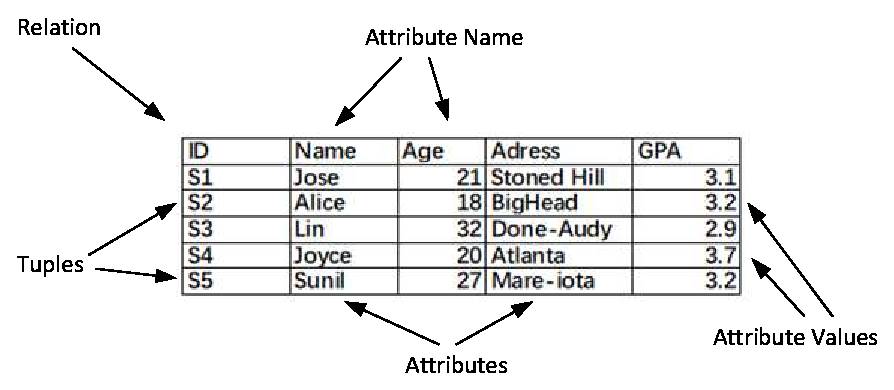
\includegraphics[width=0.8\linewidth]{handout/img/1-relation.eps}
    \caption{关系模型}\label{fig:1-relation}
\end{figure}

关系模型的单目算子包括：
\begin{itemize}
    \item $\pi$投影Projection：从关系中选择出某些属性，形成新的关系。
    \item $\sigma$选择Selection：从关系中选择出满足某些条件的元组，形成新的关系。
    \item $\tau$排序Sort：根据某个属性对关系中的元组进行排序，形成新的关系。
    \item $\delta$去重Distinct：从关系中删除重复的元组，形成新的关系。
    \item $\gamma$分组Group：根据某个属性对关系中的元组进行分组，形成新的关系。
\end{itemize}

\begin{figure}[H]
    \centering
    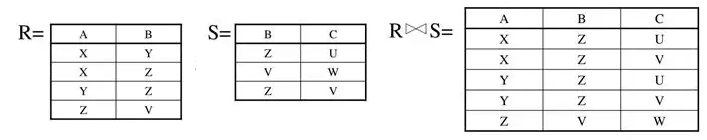
\includegraphics[width=\linewidth]{handout/img/1-join.png}
    \caption{自然连接双目算子示意图}\label{fig:1-join}
\end{figure}

双目算子包括：
\begin{itemize}
    \item $\times$笛卡尔积Cartesian Product：将两个关系的所有可能组合形成新的关系。
    \item $\bowtie$自然连接Natural Join：根据两个关系中公共属性的值进行连接，形成新的关系。
    \item $\bowtie_{c}$ $\theta$连接：根据两个关系中某个属性的值进行连接，形成新的关系。
    \item $\cup$并Union：将两个关系合并成一个新的关系，去除重复的元组。
    \item $\cap$交Intersection：从两个关系中选择出同时满足两个条件的元组，形成新的关系。
    \item $-$差Difference：从第一个关系中删除出同时出现在第二个关系中的元组，形成新的关系。
\end{itemize}

关系模型的更多内容，可以参考数据库原理课程的教材\cite{Ullman1998A}，这里仅简单回顾。

关系模型本质上是一种封闭的代数系统，其基本元素是关系Relation，关系间的运算仍然在这个代数系统上封闭。注意，虽然在实现上，关系是row的集合，但在关系运算中，Relation是基本单位而不是更小的tuple。

\begin{exercise}
    数学上，什么是系统？能举出某个学科上类似的例子吗？
\end{exercise}
\begin{exercise}
    Relation定义了单目、双目操作，这些操作够吗？一个复杂的查询总是能够通过这些操作的组合完成？
\end{exercise}
\begin{exercise}
    单目操作、双目操作，有没有三目操作？更多目操作？
\end{exercise}

\subsection{关系表达式}

一个关系$R$，经过单目操作选择后得到一个新的关系$\sigma_c(R)$，两个关系$R,S$，经过一个双目操作，得到一个新的关系$R\bowtie S$。这些算子组合起来，就可以形成一个复杂的查询表达式。例如，$R,S$关系分别先经过选择和投影，然后再连接：
$$\sigma(R) \bowtie \pi(S)$$
这些表达式称为关系表达式。关系表达式可以通过树形结构表示，如\figurename\ref{fig:1-relation-tree}所示。

\begin{figure}[H]
    \centering
    \begin{tikzpicture}[
        level distance=1cm,
        level 1/.style={sibling distance=2cm},
        level 2/.style={sibling distance=1cm},
        every node/.style={
            align=center,
            font=\small
        },
        edge from parent/.style={
            draw,
            -,
            shorten >=2pt,
            shorten <=2pt
        }
    ]
    % 根节点 - 连接操作
    \node {$\bowtie$}
        child {
            % 左子树 - 选择操作
            node {$\sigma$}
            child {
                % 叶子节点 - 关系R
                node {$R$}
            }
        }
        child {
            % 右子树 - 投影操作
            node {$\pi$}
            child {
                % 叶子节点 - 关系S
                node {$S$}
            }
        };
    \end{tikzpicture}
    \caption{关系表达式 $\sigma(R) \bowtie \pi(S)$ 的树型结构}\label{fig:1-relation-tree}
\end{figure}

关系表达式与树型结构是一一对应的，树的每个节点表示一个操作，叶子节点表示基本关系。通过这种树形结构，可以清晰地表示复杂的关系运算过程。后文在讲述查询处理时，对关系表达式和这种树型表示不加区分，二者是同一的。

在数据库原理课程里\cite{Ullman1998A}，还会介绍SQL语言，SQL语言是关系模型的一种查询语言，通过SQL语句可以方便地对关系数据库进行查询、更新、删除等操作。仅就SQL的查询功能而言，一条语句最终会对应于一个关系表达式。换句话说，SQL语言的设计目标就是能够方便地表达关系表达式。

与C语言不同，C语言是一种命令式语言，它最终的目标是将高级语言翻译成CPU上的指令序列，它的模型是一个栈指令机。SQL语言则要将查询语句翻译成关系表达式，然后选择算子的实现算法，最终生成高效的查询计划。SQL语言的设计与通用语言相比要简单得多，但要记住，它的目标是翻译成关系表达式，而不是CPU指令。

\begin{exercise}
    定义在整数集合上的加减运算，构成了一个代数系统，并由此衍生出代数表达式。代数表达式可以有许多等价表达，例如$a+(b+c)=(a+b)+c$。等价表达式有几多？类似的，关系表达式的等价表达式呢？——这暗示着什么？查询方案可以有$n$多。接下来的问题是，在特定系统中，是否存在一个最简的等价表达式，使得查询代价最低？寻找这样的最简表达式是否可行？
\end{exercise}
\begin{exercise}
    SQL查询语句得到的是什么？关系还是元组？有没有可能得到一个标量？
\end{exercise}

\section{关系数据库结构}

经过多年的发展，关系数据库的内部结构相对稳定下来，如\figurename\ref{fig:1-arch}所示。数据库内部主要有三个核心部件：执行引擎、存储引擎、事务引擎，除此外，还包含与客户对接的会话层接口等。

\begin{figure}[H]
    \centering
    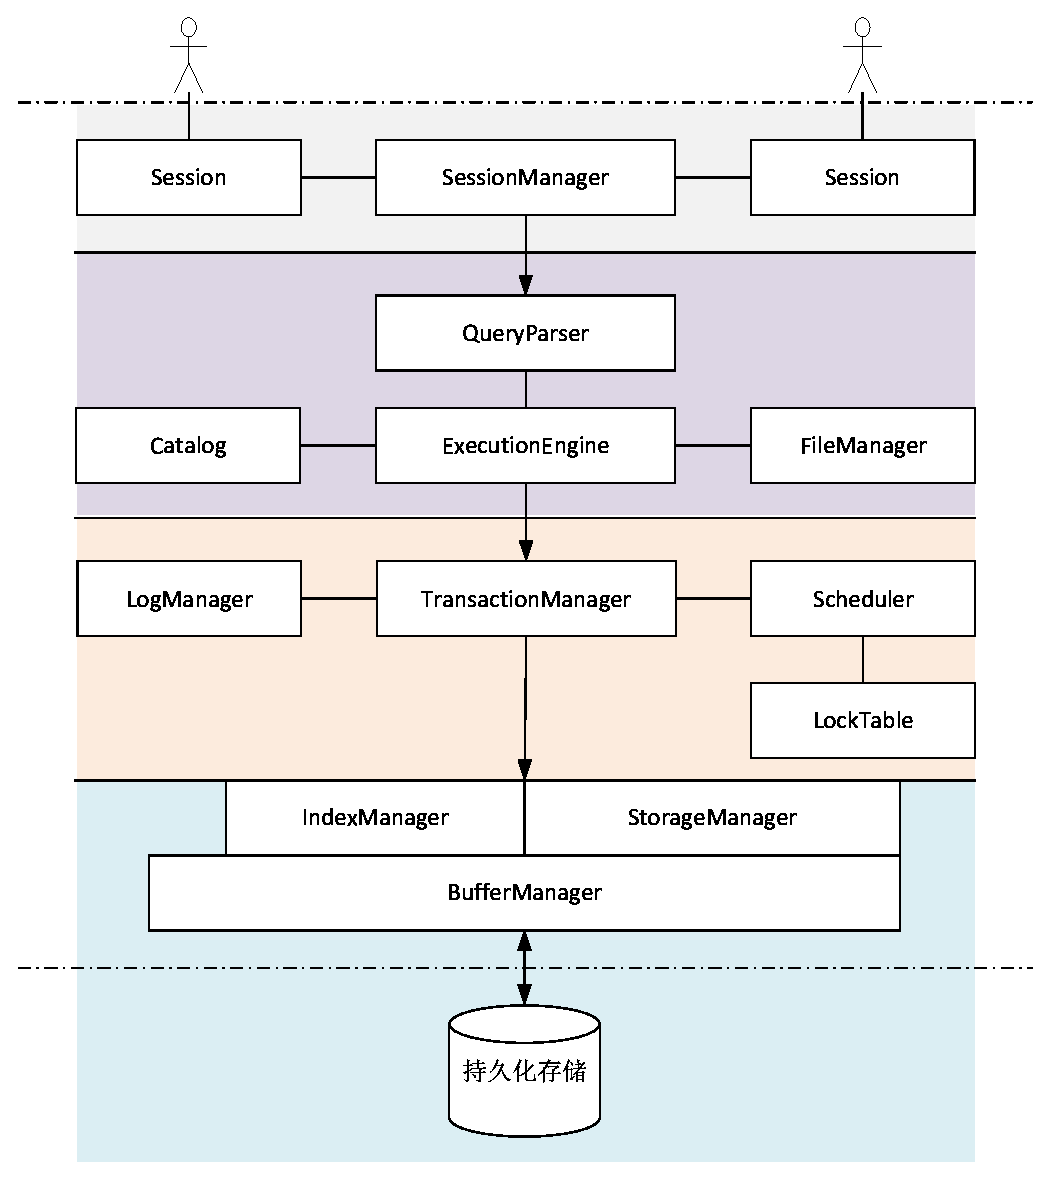
\includegraphics[width=\linewidth]{handout/img/1-arch.eps}
    \caption{关系数据库的内部结构}\label{fig:1-arch}
\end{figure}

\subsection{会话层}

一般情况下，关系数据库会部署在一个服务器上，客户端通过网络连接到数据库服务器，发送各种SQL语句。会话层负责处理客户端的连接请求，管理用户会话状态，并将SQL语句传递给执行引擎，在用户看来，会话层就是用户的代理。

有些嵌入数据库，例如SQLite，会直接将SQL语句传递给执行引擎，而不需要会话层，因为整个数据库运行在用户进程内。会话层为连续用户而设置，看成client/server模型，这里自然会有并发的问题。要保证并发的安全，要引入事务概念，这由事务引擎处理。会话层面临的问题是，如何高效地管理多个用户的连接，如何处理用户的认证和权限管理等。

完整数据库系统一般会以线程/进程形式支持多个用户的并发连接。每个用户连接会对应一个会话，会话层会负责管理这个会话的状态，包括认证、权限检查、查询处理等。随着互联网的发展，对数据库的一个挑战是如何支持大规模的并发连接。线程/进程模型在单机上支持的并发连接数量有限，未来可能会以协程方式提供会话服务。

会话层上另一个值得关注的问题是，会话代理用户执行SQL语句，它是SQL语句执行的主体，前述的执行引擎、事务引擎、存储引擎都要看成库，是会话调用执行引擎执行SQL语句。一个事务开始，中间结果、当前状态都是依附会话而存在，都要看成会话的局部变量。

\begin{exercise}
    会话接受用户SQL指令执行，将指令集看成指令流。指令流的执行是分节的，每个事务是一个小节。根据这个特性设计一个内存管理器arena，用于管理会话的局部变量。可以参考leveldb\cite{GitHubgo38:online}的arena方案。
\end{exercise}

\subsection{执行引擎}

会话收到用户的SQL语句，调用执行引擎的QueryCompiler将SQL语句编译成查询计划。这一过程包括语法分析、语义分析、逻辑优化、物理优化等阶段，最终生成一个查询计划。逻辑上，执行计划可以看成一个关系表达式的实例化，一个树型结构，叶子节点对应于关系，内部节点对应于某个关系算子，按照深度优先遍历方式执行。

以\figurename\ref{fig:1-relation-tree}为例，查询计划的执行过程如下：
\begin{enumerate}
    \item 从根节点开始，执行左子树，即选择操作$\sigma$，对关系R进行选择，得到关系R'。
    \item 然后执行右子树，即投影操作$\pi$，对关系S进行投影，得到关系S'。
    \item 最后执行连接操作$\bowtie$，将关系R'和关系S'进行连接，得到最终结果。
\end{enumerate}

在多数数据库实现中，你不会看到这种显式的树型结构执行计划，一般数据库都是用各种枚举器连接的算法。在\figurename\ref{fig:1-relation-tree}中，先调用$\sigma$算子实现函数，然后调用$\pi$算子实现函数，最后调用$\bowtie$算子实现函数。调用入口是$\bowtie$算子。——这称为火山模型volcano model。

\begin{figure}[H]
    \centering
    \begin{tikzpicture}[
        node distance=2cm,
        every node/.style={
            align=center,
            font=\small,
            minimum width=1.5cm,
            minimum height=0.8cm
        },
        operator/.style={
            rectangle,
            draw=blue!50,
            fill=blue!10,
            rounded corners=3pt,
            thick
        },
        data/.style={
            rectangle,
            draw=green!50,
            fill=green!10,
            rounded corners=3pt,
            thick
        },
        arrow/.style={
            ->,
            >=stealth,
            thick
        },
        callarrow/.style={
            ->,
            >=stealth,
            thick,
            blue,
            dashed
        },
        returnarrow/.style={
            ->,
            >=stealth,
            thick,
            red,
            dashed
        }
    ]

    % 火山模型 - 操作符调用层次
    \node[operator] (join) at (0,0) {$\bowtie$};
    \node[operator] (select) [below left=1.5cm and 1.5cm of join] {$\sigma$};
    \node[operator] (project) [below right=1.5cm and 1.5cm of join] {$\pi$};
    \node[data] (R) [below=1.5cm of select] {$R$};
    \node[data] (S) [below=1.5cm of project] {$S$};

    % 数据流箭头（实线）
    \draw[arrow] (R) -- (select);
    \draw[arrow] (S) -- (project);
    \draw[arrow] (select) -- (join);
    \draw[arrow] (project) -- (join);

    % 调用箭头（蓝色虚线）- 火山模型的核心
    \draw[callarrow] (join) to[out=180,in=90] (select);
    \draw[callarrow] (join) to[out=0,in=90] (project);
    \draw[callarrow] (select) to[out=180,in=180] (R);
    \draw[callarrow] (project) to[out=0,in=0] (S);

    % 添加标签说明
    % \node[anchor=west] at (-7,0) {\textbf{火山模型执行流程:}};
    \node[anchor=west] at (-7,0) {\textcolor{blue}{蓝色虚线}: 操作符调用};
    \node[anchor=west] at (-7,-0.5) {黑色实线: 数据流};

    \end{tikzpicture}
    \caption{火山模型（Volcano Model）执行流程}\label{fig:1-volcano-model}
\end{figure}

火山模型的执行过程可以描述为：
\begin{enumerate}
    \item 根操作符$\bowtie$开始执行，调用其子操作符$\sigma$和$\pi$
    \item 每个子操作符递归调用其子操作符（叶子节点直接访问数据）
    \item 数据从叶子节点逐级向上返回
    \item 每个操作符处理接收到的数据，生成新的数据
    \item 最终结果从根操作符输出
\end{enumerate}

这种模型之所以称为火山，是因为数据从底层向上喷发，经过各个操作符的处理，最终从顶部输出结果。火山模型的一个重要特点是每个操作符都实现了统一的接口，如open、next、close等。对于流式处理，火山模型可以使得某个tuple连续经过多个算子的处理，一次性输出结果，减少中间结果的存储开销，提高查询效率。火山模型的问题是，对指令缓存不友好，因为每个操作符调用都是函数调用，会导致频繁的上下文切换，影响CPU指令缓存的命中率。

\begin{exercise}
    构思一种方案，改善火山模型的指令缓存不友好问题。
\end{exercise}

QueryCompiler如何将SQL语句翻译成查询计划？SQL语言比较小巧，它的目标是最终将SQL语句翻译成关系表达式，然后选择具体的算子实现算法，最终生成查询计划。SQL语言的设计与通用语言相比要简单得多，但要记住，它的目标是翻译成关系表达式，而不是CPU指令。

\subsection{存储引擎}

关系数据库的存储引擎主要包含三个方面的功能：底层存储组织、索引结构、以及buffer缓冲。底层存储组织负责将关系数据存储在磁盘上，通常采用页page的方式进行存储，每个页包含多个记录record。索引结构用于加速数据的查询，多数数据库采用btree作为索引结构。buffer缓冲用于缓存最近访问的数据页，减少磁盘I/O操作，提高查询性能。

在\figurename\ref{fig:1-arch}中，会话执行SQL语句的执行计划，按照火山模型调用next迭代接口，访问某个关系$R$的元组tuple。返回tuple的过程有点长，存储引擎根据$R$名到数据库元信息catalog中找到存储的文件名，打开文件，这里有文件管理的问题。文件打开，对应于一个文件描述符fd。这里我们还不了解btree索引结构，将它想象成一个$f(x)$函数，输入tuple的主键key，输出tuple在文件中的偏移量offset。拿到这个offset后，到缓冲管理器里根据$fd:offset$查找page，如果page不在缓冲区，就从磁盘加载page到缓冲区。页面调入缓冲后，在page内部找到tuple对应的记录，解析后返回给执行引擎。

\begin{figure}[H]
    \centering
    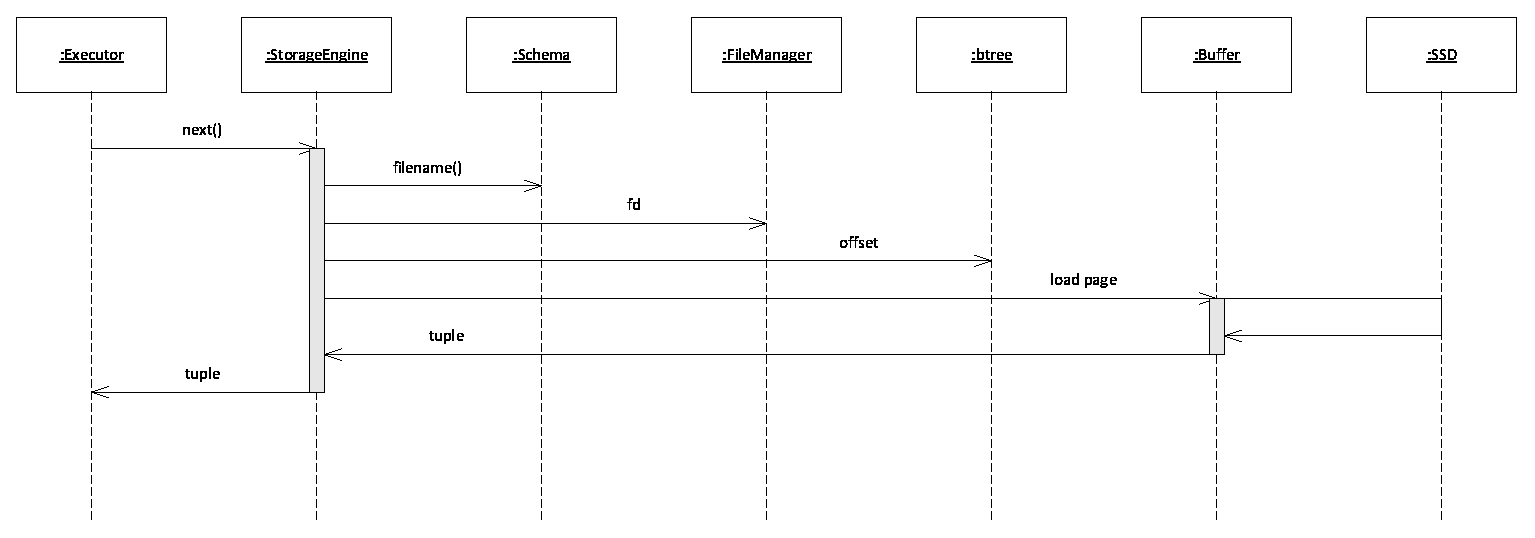
\includegraphics[width=1.2\linewidth]{handout/img/1-tuple.eps}
    \caption{存储引擎返回tuple过程}\label{fig:1-tuple}
\end{figure}

\begin{exercise}
    假设会话层用协程实现，协程模型为$m:n$，有$n$个线程，有远多于$m>>n$的协程，当协程等待异步结果，协程被挂起。编写open\_page()函数伪码，从HDD/SSD上读出page到缓冲区。
\end{exercise}

\subsection{事务引擎}

事务是数据库领域的一个抽象概念，一个事务看成是一组执行流，将数据库的数据看成公共的资源，事务对公共资源的访问要遵循一定的规则，否则会导致不一致问题，例如某个事务正在修改某个银行账户上的余额，另一个事务正在读取这个余额，如果不加控制，就会导致读取到不一致的数据。

事务的概念其实并不仅限于数据库系统，以一个web服务为例，它后台挂着一个数据库，通过web服务暴露API给用户使用。用户连接数据库后，发起一个事务，从物理边界上看，事务涵盖着用户端、web服务端、数据库端多个部分，要将这些部分看成一个整体，才能理解事务的意义。

事务具有原子性、一致性、隔离性、持久性（ACID）等特性。原子性指事务要么全部成功，要么全部失败；一致性指事务执行前后，数据库要保持一致的状态；隔离性指多个事务并发执行时，要相互隔离，避免互相干扰；持久性指事务一旦提交，其结果要永久保存。

ACID原则中，最难理解的是一致性，何谓一致的状态？一致性其实是用户的约束，不同的系统有不同的约束。站在数据库的角度，如何保证一致性？数据库的数据访问抽象为read/write两种操作，数据库的一致性要保证多个事务并发执行时，read/write是一致的。

\begin{exercise}
    事务的原子性要求事务执行得非常快？与CPU的原子指令有何区别？
\end{exercise}

事务引擎主要处理两方面的工作：事务并发、故障恢复。并发目前常用的方案是：基于锁的并发控制、基于时间戳的并发控制。故障恢复则主要通过日志记录和检查点机制实现。

在\figurename\ref{fig:1-arch}中，事务引擎的主要工作是控制会话的执行流。在实现中，事务代码一般是嵌入到执行引擎、存储引擎代码中，控制事务的开始、提交、回滚等操作。以\figurename\ref{fig:1-relation-tree}为例，当读取关系$R$，会对$R$的每个tuple加锁，防止其他事务修改$R$。当读取关系$S$，会对$S$的每个tuple加锁，防止其他事务修改$S$。当事务提交时，会释放所有加的锁。

